\documentclass[a4paper,12pt]{article}
\usepackage[left=2cm,right=2cm,top=2cm,bottom=2cm]{geometry} % Do ustawień marginesów
\usepackage{multicol} % Dla podziału na kolumny
\usepackage{ragged2e} % Dla justowania tekstu
\usepackage{graphicx} % Required for inserting images
\usepackage{float}
\usepackage{caption}
\usepackage{amsmath} % Math formulas
\usepackage{amssymb} % Symbols
\usepackage[svgnames]{xcolor}
\usepackage[colorlinks=true, urlcolor=blue, linkcolor=black, citecolor=orange]{hyperref} % Hyperlinks
\usepackage{polski} % Polish language
\usepackage[utf8]{inputenc} % Text encoding
\usepackage{enumitem} % Pakiet do elastycznego sterowania listami
\usepackage{indentfirst}
\usepackage{array}
\usepackage{longtable}

\setlist[itemize]{itemsep=0pt, topsep=0pt}

\begin{document}

% Górna część strony
\noindent
\begin{minipage}{0.5\textwidth}
    \raggedright
    \textbf{Piotr Durniat} \\
    I rok, Fizyka \\
    Wtorek, 8:00-10:15 \\
    \vspace{0.5cm}
    \vspace{0.5cm}
\end{minipage}%
\begin{minipage}{0.5\textwidth}
    \raggedleft
    Data wykonania pomiarów: \\
    06.05.2025 \\
    \vspace{0.5cm}
    Prowadząca: \\
    dr Iwona Mróz
\end{minipage}

% Tytuł ćwiczenia
\vspace{2cm}
\begin{center}
    \LARGE \textbf{Ćwiczenie nr 29} \\[0.5cm]
    \Large \textbf{Anomalia rozszerzalności cieplnej wody}
\end{center}

\vspace{1cm}
\noindent

\tableofcontents
\newpage

% ---------- WSTĘP TEORETYCZNY ----------
\section{Wstęp teoretyczny}

% ---------- OPIS DOŚWIADCZENIA ----------
\section{Opis doświadczenia}

% ---------- OPRACOWANIE WYNIKÓW POMIARÓW ----------
\section{Opracowanie wyników pomiarów}

% ---------- TABELE ----------
\subsection{Tabele pomiarowe}

\begin{longtable}{|c|c|c|}
    \hline
    $T$ [$^\circ$C] & \multicolumn{2}{c|}{$h$ [mm]} \\
    \hline
    & Seria 1 & Seria 2 \\
    \hline
    \endhead
    11.0 & 80 & 71 \\
    10.8 & 77 & 70 \\
    10.6 & 75 & 68 \\
    10.4 & 74 & 66 \\
    10.2 & 72 & 64 \\
    10.0 & 69 & 62 \\
    9.8  & 68 & 60 \\
    9.6  & 66 & 58 \\
    9.4  & 64 & 56 \\
    9.2  & 63 & 55 \\
    9.0  & 61 & 54 \\
    8.8  & 61 & 51 \\
    8.6  & 60 & 51 \\
    8.4  & 56 & 49 \\
    8.2  & 55 & 48 \\
    8.0  & 53 & 46 \\
    7.8  & 52 & 44 \\
    7.6  & 51 & 44 \\
    7.4  & 50 & 43 \\
    7.2  & 49 & 41 \\
    7.0  & 47 & 40 \\
    6.8  & 46 & 39 \\
    6.6  & 45 & 37 \\
    6.4  & 44 & 37 \\
    6.2  & 43 & 36 \\
    6.0  & 42 & 40 \\
    5.8  & 42 & 36 \\
    5.6  & 42 & 34 \\
    5.4  & 40 & 32 \\
    5.2  & 40 & 32 \\
    5.0  & 39 & $<30$ \\
    4.8  & 38 & $<30$ \\
    4.6  & 38 & $<30$ \\
    4.4  & 38 & $<30$ \\
    4.2  & 37 & $<30$ \\
    4.0  & 37 & $<30$ \\
    3.8  & 37 & $<30$ \\
    3.6  & 37 & $<30$ \\
    3.4  & 37 & $<30$ \\
    3.2  & 37 & $<30$ \\
    3.0  & 37 & $<30$ \\
    2.8  & 37 & 30 \\
    2.6  & 37 & 30 \\
    2.4  & 38 & 30 \\
    2.2  & 38 & 32 \\
    2.0  & 38 & 33 \\
    1.8  & 39 & 34 \\
    1.6  & 39 & 34 \\
    1.4  & 40 & 35 \\
    1.2  & 40 & 36 \\
    1.0  & 41 & 37 \\
    0.8  & 41 & 38 \\
    0.6  & 42 & 39 \\
    0.4  & 43 & 40 \\
    0.2  & 43 & 41 \\
    \hline
    \caption{Wyniki pomiarów wysokości słupa wody w zależności od temperatury}
    \label{tab:pomiary_wysokosci}
\end{longtable}

Średnica wewnętrzna kapilary wynosi $d = 1{,}7 $ mm.

% ---------- OBLICZENIA ----------
\subsection{Zmiana objętości wody}

Na podstawie zmierzonej wysokości słupa wody obliczono objętość wody w kapilarze według wzoru:
\begin{equation}
    V = \pi \cdot \frac{d^2}{4} \cdot h
\end{equation}

gdzie $d = 1,7$ mm jest średnicą wewnętrzną kapilary, a $h$ jest wysokością słupa wody.

Obliczono również zmianę objętości $\Delta V$ względem objętości początkowej (dla temperatury 11,0°C):
\begin{equation}
    \Delta V = V - V_{11,0°C}
\end{equation}

\begin{table}[H]
    \centering
    \caption{Wartości objętości wody oraz zmiany objętości (wybrane temperatury)}
    \label{tab:objetosci}
    \begin{tabular}{|c|c|c|c|c|}
        \hline
        $T$ [$^\circ$C] & $V_1$ [m$^3$] & $V_2$ [m$^3$] & $\Delta V_1$ [m$^3$] & $\Delta V_2$ [m$^3$] \\
        \hline
        11,0 & 1,82$\cdot$10$^{-7}$ & 1,61$\cdot$10$^{-7}$ & 0 & 0 \\
        10,0 & 1,57$\cdot$10$^{-7}$ & 1,41$\cdot$10$^{-7}$ & -2,50$\cdot$10$^{-8}$ & -2,04$\cdot$10$^{-8}$ \\
        9,0 & 1,38$\cdot$10$^{-7}$ & 1,23$\cdot$10$^{-7}$ & -4,31$\cdot$10$^{-8}$ & -3,86$\cdot$10$^{-8}$ \\
        8,0 & 1,20$\cdot$10$^{-7}$ & 1,04$\cdot$10$^{-7}$ & -6,13$\cdot$10$^{-8}$ & -5,67$\cdot$10$^{-8}$ \\
        7,0 & 1,07$\cdot$10$^{-7}$ & 9,08$\cdot$10$^{-8}$ & -7,49$\cdot$10$^{-8}$ & -7,04$\cdot$10$^{-8}$ \\
        6,0 & 9,53$\cdot$10$^{-8}$ & 9,08$\cdot$10$^{-8}$ & -8,63$\cdot$10$^{-8}$ & -7,04$\cdot$10$^{-8}$ \\
        5,0 & 8,85$\cdot$10$^{-8}$ & 6,81$\cdot$10$^{-8}$ & -9,31$\cdot$10$^{-8}$ & -9,31$\cdot$10$^{-8}$ \\
        4,0 & 8,40$\cdot$10$^{-8}$ & 6,81$\cdot$10$^{-8}$ & -9,76$\cdot$10$^{-8}$ & -9,31$\cdot$10$^{-8}$ \\
        3,0 & 8,40$\cdot$10$^{-8}$ & 6,81$\cdot$10$^{-8}$ & -9,76$\cdot$10$^{-8}$ & -9,31$\cdot$10$^{-8}$ \\
        2,0 & 8,63$\cdot$10$^{-8}$ & 7,49$\cdot$10$^{-8}$ & -9,53$\cdot$10$^{-8}$ & -8,63$\cdot$10$^{-8}$ \\
        1,0 & 9,31$\cdot$10$^{-8}$ & 8,40$\cdot$10$^{-8}$ & -8,85$\cdot$10$^{-8}$ & -7,72$\cdot$10$^{-8}$ \\
        0,2 & 9,76$\cdot$10$^{-8}$ & 9,31$\cdot$10$^{-8}$ & -8,40$\cdot$10$^{-8}$ & -6,81$\cdot$10$^{-8}$ \\
        \hline
    \end{tabular}
\end{table}

Pełne dane objętości dla wszystkich pomiarów przedstawiono na wykresie (Rys.~\ref{fig:height_vs_temperature}). Można zauważyć, że woda osiąga najmniejszą objętość (największą gęstość) w okolicy temperatury 4°C, co potwierdza zjawisko anomalii rozszerzalności cieplnej wody.

% ---------- NIEPEWNOŚCI ----------
\section{Ocena niepewności pomiaru}

% ---------- WNIOSKI ----------
\section{Wnioski}

\newpage
% ---------- WYKRESY ----------
\section{Wykresy}

\begin{figure}[H]
    \centering
    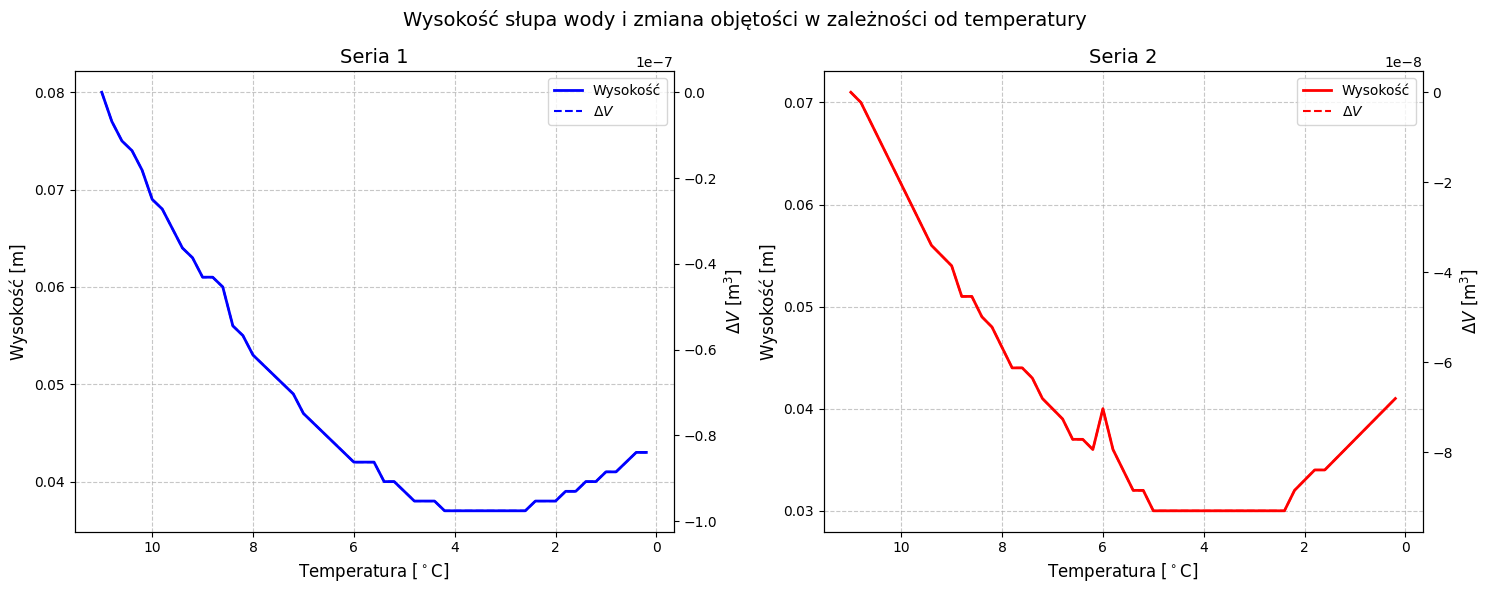
\includegraphics[width=0.9\textheight,angle=90]{height_vs_temperature.png}
    \caption{Wysokość słupa wody w zależności od temperatury}
    \label{fig:height_vs_temperature}
\end{figure}


\bibliographystyle{plain}
\bibliography{bibliography}

\end{document}
